\begin{figure}[!htbp]
  \centering
  \begin{subfigure}[b]{0.4\textwidth}
    \centering
    \tikzsetnextfilenamesafe{Chapter4/3D/calibrated/pdf}
    \begin{tikzpicture}
      \begin{axis}[
          width=\textwidth,
          height=1\textwidth,
          xlabel=$l^*$,ylabel=estimated PDF,
          ymin=0,ymax=0.5,
          xmin=0,xmax=15,
          legend style={at={(0.95,0.95)},anchor=north east},
          legend style={nodes={scale=1, transform shape}},
          legend style={fill=none, draw=none},
          legend cell align={left},
          every axis plot/.append style={thick}
        ]
        \addplot [color=black] table [x expr=\thisrowno{0},y expr=\thisrowno{1}]{Chapter4/data/3D/calibrated_pdf.csv};
        \addplot [color=red] table [x expr=\thisrowno{0},y expr=\thisrowno{2}]{Chapter4/data/3D/calibrated_pdf.csv};
        \legend{experiment,simulation}
      \end{axis}
    \end{tikzpicture}
    \caption{}
  \end{subfigure}
  \begin{subfigure}[b]{0.27\textwidth}
    \centering
    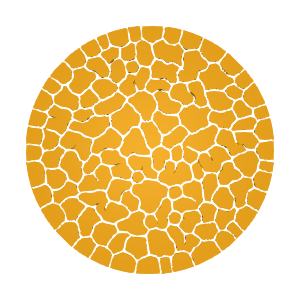
\includegraphics[width=\textwidth]{Chapter4/figures/3D/d_4.png}
    \vspace{10pt}
    \caption{}
  \end{subfigure}
  \begin{subfigure}[b]{0.25\textwidth}
    \centering
    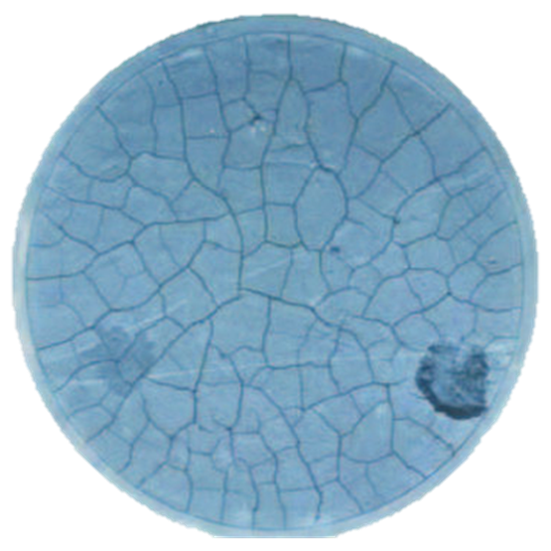
\includegraphics[width=\textwidth]{Chapter4/figures/3D/4mm_exp.png}
    \vspace{12pt}
    \caption{}
  \end{subfigure}
  \caption[Comparison between the simulation and the experiment after calibration.]{(a) Estimated PDFs of the dimensionless fragment sizes extracted from the experimental result and the calibrated stochastic model. (b) Fracture morphology obtained using the calibrated fracture properties. (c) Photograph of cracks in the mining waste. }
  \label{fig: Chapter4/3D/calibrated}
\end{figure}
